\chapter{Advanced Quantum Mechanics Lecture 3: Angular Momentum, Central Forces, and Ladder Operators}

This lecture develops the angular momentum framework into a practical spectral tool for central-force quantum problems, then recasts the same ladder-operator method for the harmonic oscillator. The momentum-space intuition from classical orbital motion appears first through geometry, then becomes algebraic structure: angular sectors are organized by multiplets, each carrying fixed \(\ell\), and within each sector one solves a one-dimensional radial problem. The logic is to separate the quantum dynamics into angular and radial pieces, classify angular sectors with \(L_\pm\) algebra, and read off degeneracy and energy ordering before solving detailed differential equations.

\section{Setup: central-force motivation and angular structure}
In a central force field the potential depends only on the radial coordinate, \(V(r)\). A natural variable split is \((r,\theta,\phi)\), and the angular dependence carries the orbital angular momentum content while the radial part carries the remaining dynamics.

Classically the orbital momentum is
\[
\mathbf L=\mathbf r\times \mathbf p
\]
and is conserved for rotationally invariant potentials. Quantum mechanically this conservation is represented by commuting angular momentum operators with the central-force Hamiltonian. The wavefunction for one particle in ordinary space is \(\psi(\mathbf r)=\psi(r,\theta,\phi)\), and in a central field the angular dependence is the part controlled by \(\mathbf L\). The orbit in configuration space lies in a plane for fixed \(\mathbf L\), but in quantum mechanics the full state is still a wavefunction in three dimensions; the “plane” idea is implemented as angular-sector decomposition.

\section{Warm-up in two dimensions and extension to \(3\)D angular modes}
To build the idea, recall the two-dimensional case with coordinates \((r,\theta)\). If \(L_z\) is the generator of rotations in the plane, then (with \(\hbar=1\) temporarily)
\[
\hat L_z=-i\hbar\frac{\partial}{\partial\theta}.
\]
Solving \(\hat L_z\psi=\hbar m\psi\) yields
\[
\psi(r,\theta)=\chi(r)e^{im\theta}, \qquad m\in\mathbb Z.
\]
The integer condition follows from single-valuedness:
\[
\psi(r,\theta+2\pi)=\psi(r,\theta)\implies e^{i m 2\pi}=1\implies m\in\mathbb Z.
\]

\paragraph{Consequence.}
For fixed \(m\), only the radial profile \(\chi(r)\) changes with dynamics; angular dependence is fixed by \(e^{im\theta}\). In three dimensions the same organizing idea persists: radial part times angular eigenfunctions on the sphere,
\[
\psi(r,\theta,\phi)=R_{n\ell}(r)\,Y_\ell^m(\theta,\phi),
\]
with \(m\) the magnetic quantum number and \(\ell\) the fixed angular-momentum multiplet label.

\begin{figure}
\centering
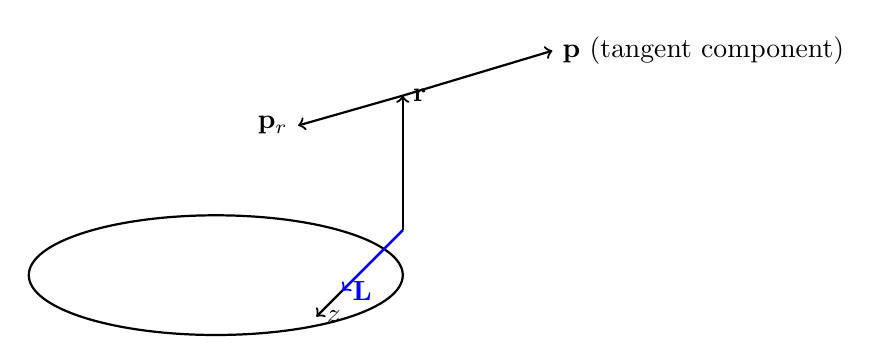
\begin{tikzpicture}[scale=0.95]
  \draw[thick,->] (0,0) -- (0,0,3) node[right] {$z$};
  \draw[thick] (-2.5,-0.6) ellipse (2.5 and 0.8);
  \draw[thick,->] (0,0) -- (0,1.8) node[right] {$\mathbf r$};
  \draw[thick,->] (0,1.8) -- (2.0,2.4) node[right] {$\mathbf p$ (tangent component)};
  \draw[thick,->] (0,1.8) -- (-1.4,1.4) node[left] {$\mathbf p_r$};
  \draw[->,blue,thick] (0,0) -- (0,0,2.1) node[right] {$\mathbf L$};
\end{tikzpicture}
\caption{Orbit-plane geometry in a central-force problem and its momentum decomposition into radial and angular parts.}
\end{figure}

\section{Angular-momentum commutators and ladder operators}
We take the standard angular momentum algebra
\[
[\hat L_x,\hat L_y]=i\hbar \hat L_z,\qquad
[\hat L_y,\hat L_z]=i\hbar \hat L_x,\qquad
[\hat L_z,\hat L_x]=i\hbar \hat L_y
\]
(\textit{transcript-verified}).

Define
\[
\hat L_\pm=\hat L_x\pm i\hat L_y.
\]
Then
\[
[\hat L_z,\hat L_\pm]=\pm\hbar \hat L_\pm,
\]
so if \(\hat L_z|\ell,m\rangle=\hbar m|\ell,m\rangle\), then
\[
\hat L_z(\hat L_\pm|\ell,m\rangle)=\hbar(m\pm1)\hat L_\pm|\ell,m\rangle,
\]
and thus \(\hat L_\pm\) shifts \(m\) by \(\pm1\).

\paragraph{Termination and finite ladder.}
Repeatedly applying \(\hat L_+\) on a given state must terminate at top \(m_{\max}\), because otherwise one gets an infinite chain not supported by physical finite norm sectors in this setting (the standard angular-momentum argument). The only nonzero possibility is
\[
\hat L_+|\ell,m_{\max}\rangle=0,\qquad
\hat L_-|\ell,m_{\min}\rangle=0.
\]
By symmetry between \(+\hat z\) and \(-\hat z\), this implies a symmetric ladder:
\[
m_{\min}=-\ell,\qquad m_{\max}=+\ell,\qquad m=-\ell,-\ell+1,\ldots,\ell.
\]
Hence one has \(2\ell+1\) states per multiplet.

\begin{figure}
\centering
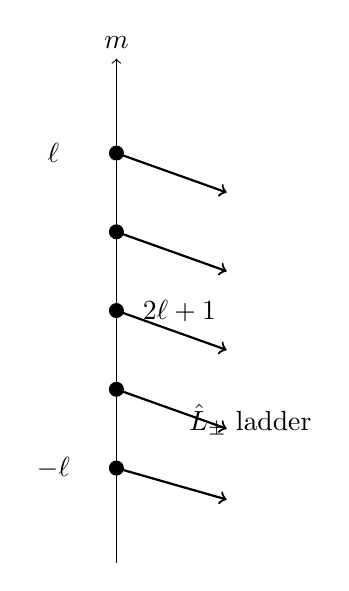
\begin{tikzpicture}[scale=1]
  \draw[->] (0,-3.2) -- (0,3.2) node[above] {$m$};
  \foreach \y in {-2,-1,0,1,2}
    \draw[fill=black] (0,\y) circle (2.5pt);
  \node at (-0.8,2.0) {$\ell$};
  \node at (-0.8,-2.0) {$-\ell$};
  \node at (0.8,0.0) {$2\ell+1$};
  \draw[->,thick] (0,2.0) -- (1.4,1.5);
  \draw[->,thick] (0,1.0) -- (1.4,0.5);
  \draw[->,thick] (0,0) -- (1.4,-0.5);
  \draw[->,thick] (0,-1.0) -- (1.4,-1.5);
  \draw[->,thick] (0,-2.0) -- (1.4,-2.4);
  \node at (1.7,-1.4) {$\hat L_\pm$ ladder};
\end{tikzpicture}
\caption{The \(m\)-ladder for fixed \(\ell\), terminated at \(m=\pm\ell\).}
\end{figure}

\section{Multiplets and the value of \(\hat L^2\)}
For fixed \(\ell\), all states in one ladder are degenerate in \(\hat L^2\). Write
\[
\hat L^2=\hat L_x^2+\hat L_y^2+\hat L_z^2
=\hat L_-\hat L_+ + \hat L_z^2+\hbar \hat L_z
\]
(\textit{transcript-verified}, up to operator-order presentation). Acting on the top state,
\[
\hat L_+|\ell,\ell\rangle=0
\]
and therefore
\[
\hat L^2|\ell,\ell\rangle
=(\hat L_-\hat L_++\hat L_z^2+\hbar\hat L_z)|\ell,\ell\rangle
=\hbar^2\ell(\ell+1)|\ell,\ell\rangle.
\]

Since
\[
[\hat L^2,\hat L_\pm]=0,
\]
the same eigenvalue applies to all states generated by \(\hat L_\pm\) in the multiplet:
\[
\hat L^2|\ell,m\rangle=\hbar^2\ell(\ell+1)|\ell,m\rangle,\qquad m=-\ell,\ldots,\ell.
\]
This is the quantum correction relative to the classical form \(L_{\text{class}}^2=\ell^2\hbar^2\): in quantum mechanics magnitude becomes \(\ell(\ell+1)\hbar^2\).

\begin{proposition}
For a fixed multiplet label \(\ell\), \(\hat L^2\) is constant across all \(m\in\{-\ell,\ldots,\ell\}\), while \(\hat L_z\) separates them by integer steps.
\end{proposition}
\begin{proof}
Use \([\hat L^2,\hat L_\pm]=0\), and \(\hat L_\pm\) moves only \(m\). Since \(\hat L_\pm\) connects all states inside the finite ladder, \(\hat L^2\) has one common eigenvalue on that ladder.
\end{proof}

\section{From \(\mathbf L\) to radial dynamics: the central-force Hamiltonian}
Write the Schrödinger Hamiltonian
\[
\hat H=\frac{\hat{\mathbf p}^2}{2m}+V(r).
\]
Classically this decomposes as radial plus angular momentum kinetic pieces:
\[
\hat{\mathbf p}^2=\hat p_r^2+\hat p_\theta^2+\hat p_\phi^2
\]
(with the transverse part captured by \(\hat L^2=r^2\hat p_\perp^2\) in \(3\)D spherical decomposition). For central problems this is re-expressed as
\[
\hat H=\frac{\hat p_r^2}{2m}+\frac{\hat L^2}{2mr^2}+V(r).
\]
When acting in one \(\ell\)-sector, replace \(\hat L^2\to \hbar^2\ell(\ell+1)\):
\[
\hat H_{\ell,\mathrm{rad}}
=\frac{\hat p_r^2}{2m}+\frac{\hbar^2\ell(\ell+1)}{2mr^2}+V(r).
\]
The factorization used in textbooks then gives the standard one-dimensional form
\[
\left[-\frac{\hbar^2}{2m}\frac{d^2}{dr^2}
+V(r)+\frac{\hbar^2\ell(\ell+1)}{2mr^2}\right]u_{n_r\ell}(r)=E_{n_r\ell}\,u_{n_r\ell}(r),
\]
where \(u(r)=rR_{n_r\ell}(r)\) (up to convention).

\paragraph{Interpretation.}
\(\frac{\hbar^2\ell(\ell+1)}{2mr^2}\) is a centrifugal barrier. For \(\ell=0\) it vanishes; for \(\ell>0\) it strongly suppresses near-\(r=0\) probability and raises the effective low-energy radial scale.

\begin{figure}
\centering
\begin{tikzpicture}[scale=1.1]
  \draw[->] (0,0) -- (7,0) node[right] {$r$};
  \draw[->] (0,0) -- (0,3.1) node[above] {$V_{\text{eff}}(r)$};
  \draw[thick,domain=0.5:6.5,smooth,variable=\x] plot ({\x},{2.2/(\x*\x)+1.1});
  \draw[thick,dashed,domain=0.5:6.5,smooth,variable=\x] plot ({\x},{1.2-(0.08*(\x-1)*(\x-1))});
  \draw[thick,blue] (0.5,2.5) -- (6.5,1.6) node[right] {$V_{\text{eff}}=V(r)+\frac{\ell(\ell+1)\hbar^2}{2mr^2}$};
  \node at (4.5,1.0) {$V(r)$};
  \node at (3.6,0.3) {allowed bound region};
\end{tikzpicture}
\caption{Schematic effective potential for \(\ell>0\): centrifugal barrier plus central attraction.}
\end{figure}

\section{Node counting and atomic-like spectral organization}
For a fixed \(\ell\), the radial equation has a one-dimensional spectral ladder. In broad terms, the node count provides ordering:
\[
n_r=0,1,2,\ldots
\]
for bound states in a given \(\ell\)-sector, with larger \(n_r\) typically at higher energy. This is standard in 1D Schrödinger problems and was emphasized as a practical organizing principle.

Each level in an \(\ell\)-sector carries magnetic degeneracy \(2\ell+1\). A compact summary is
\begin{table}[h]
\centering
\begin{tabular}{c c c}
\hline
\(\ell\) & \(m\)-values & degeneracy \\
\hline
0 & \(0\) & \(1\) \\
1 & \(-1,0,1\) & \(3\) \\
2 & \(-2,-1,0,1,2\) & \(5\) \\
3 & \(-3,\dots,3\) & \(7\) \\
\hline
\end{tabular}
\caption{Magnetic multiplicity for fixed \(\ell\).}
\end{table}

For each \(\ell\), adding \(\ell\) increases the centrifugal term, so whole towers shift upward relative to smaller \(\ell\), and states with more nodes rise up within the same \(\ell\)-sector.

\section{Coulomb potential: special degeneracy and its fragility}
For \(V(r)=-\kappa/r\), many features are qualitatively visible from the same effective picture: the \(1/r\) tail and \(1/r^2\) barrier combine to produce bound radial ladders and a characteristic pattern. In this ideal nonrelativistic case one finds near-accidental degeneracies across different \((n_r,\ell)\) sets (approximate principal-like grouping), so levels with different \(\ell\) can coincide more often than expected.

This coincidence is exact only for the ideal \(1/r\) law in this framework, not for all atoms. Real systems include:
\begin{itemize}
\item relativistic corrections,
\item finite nucleus size,
\item electron spin and associated couplings,
\item and other many-body/environmental effects.
\end{itemize}
These perturb that degeneracy, a point stressed as “special/fragile accident” versus robust structure.

\section{Harmonic oscillator: a second ladder-operator victory}
A useful template repeats the same logic. Set \(m=1\) for simplicity:
\[
\hat H=\frac{\hat p^2}{2}+\frac{1}{2}\omega^2\hat x^2.
\]
Define
\[
\hat a_\pm=\frac{1}{\sqrt{2\hbar\omega}}\left(\mp i\hat p + \omega \hat x\right),
\qquad
[\hat a_-,\hat a_+]=1
\]
(\textit{transcript-verified}/\textit{standard completion}).

Then
\[
\hat H=\hbar\omega\left(\hat a_+\hat a_-+\frac12\right)
=\hbar\omega(\hat N+\tfrac12),
\qquad
\hat N\equiv \hat a_+\hat a_-.
\]

From the commutators,
\[
[\hat N,\hat a_+]=\hat a_+,\qquad [\hat N,\hat a_-]=-\hat a_-.
\]
So \(\hat a_+\) raises \(N\)-eigenvalue by one and \(\hat a_-\) lowers it by one. To avoid negative or unbounded descent, one imposes a ground state \(|0\rangle\) with
\[
\hat a_-|0\rangle=0.
\]
Then one gets
\[
\hat N|n\rangle=n|n\rangle,\qquad n=0,1,2,\ldots
\]
and therefore
\[
E_n=\hbar\omega\left(n+\frac12\right).
\]
The \(+\frac12\hbar\omega\) term is the zero-point energy.

This is the same motif as for angular momentum: a factorization exposes stepping operators, and a boundary/termination condition quantizes the spectrum.

\begin{figure}
\centering
\begin{tikzpicture}[scale=1]
  \draw[->] (0,0) -- (0,3.5) node[above] {$E$};
  \draw[->] (0,0) -- (7,0) node[right] {$n$};
  \foreach \x in {0.8,1.6,2.4,3.2,4.0}
    \draw[thick] (\x,0.8+\0.25*\x) -- (\x+0.35,0.8+0.25*\x);
  \foreach \x in {0,1,2,3}
    \draw (\x*0.8+0.8,0.8+0.25*(\x*0.8+0.8)) -- +(0,0.35);
  \foreach \y in {0.9,1.15,1.4,1.65,1.9}
    \node at (7.1,\y) {$(n+\frac12)\hbar\omega$};
  \node at (3.4,3.1) {HO ladder via \(a_+\) and \(a_-\)};
\end{tikzpicture}
\caption{Heuristic sketch of equally spaced oscillator energies from ladder stepping.}
\end{figure}

\section{Summary}
This lecture’s central message is that angular momentum structure is a computational architecture: angular dependence is classified by \(\hat L_z\) and \(\hat L^2\), ladder operators organize finite multiplets, and central-force Hamiltonians reduce to radial equations with an \(\ell\)-dependent centrifugal barrier. The same algebraic strategy reappears in the harmonic oscillator through factorization, showing how commutator structure and step operators produce quantized spectra with a ground-state boundary condition.

Based on Leonard Susskind’s Advanced Quantum Mechanics Lecture 3 (2013 Fall), notes curated by LazyingArt LLC.